\documentclass[aspectratio=169,xcolor=dvipsnames]{beamer}
\setbeamerfont{footnote}{size=\tiny}
\usetheme{SimpleDarkBlue}

\usepackage{amssymb}
\usepackage{amsmath}
\usepackage{mathtools}
\usepackage{tikz-cd}
\usepackage{tikz}
\usepackage{subcaption} 

\usetikzlibrary{decorations.pathreplacing,calc, positioning}
\colorlet{BraceColor}{HeaderBand}   % draw colour for braces
\colorlet{BubbleBG}{HeaderBand}     % fill colour for speech bubbles
\colorlet{BubbleText}{TextSoft}     % readable off‑white text
\definecolor{BGCanvas}{HTML}{36454f}
\definecolor{AccentLight}{HTML}{A7CCED}
\definecolor{BlockHeadExample}{HTML}{97b8c2}
\definecolor{BlockHeadAlerted}{HTML}{7a9ca7}
\definecolor{BlockHeadDefault}{HTML}{b0d6df}

\usepackage{hyperref}
\usepackage{graphicx}
\usepackage{booktabs}
\usepackage{multirow}

\newcommand{\reals}{\mathbb{R}}
\newcommand{\complex}{\mathbb{C}}
\newcommand{\integers}{\mathbb{Z}}
\newcommand{\rationals}{\mathbb{Q}}
\newcommand{\naturals}{\mathbb{N}}
\renewcommand{\thefootnote}{}


% chktex warning suppression
% chktex-file 44
% chktex-file 42
% chktex-file 12
% chktex-file 8
% chktex-file 2

\title{An Epidemiological Mixed-Integer Nonlinear Programming Framework for Vaccine Modeling and Patient Allocation During Pandemics}
\author{Alexander DeLise$^1$, \underline{Seyedreza Abazari$^2$}, and Dr. Arda Vanli$^2$}
\institute{$^1$Florida State University, $^2$FAMU-FSU College of Engineering} %\\ 10th North American Conference on Industrial Engineering and Operations Management}
%\date{June 17-19, 2025}
\titlegraphic{
\includegraphics[height=1.5cm]{logos/famu.png}
\includegraphics[height=1.5cm]{logos/fsu.png}} 


\begin{document}

\begin{frame}\titlepage\end{frame}

\begin{frame}{Overview}
    \tableofcontents
\end{frame}

%---------------------------------------------
\section{Preliminaries}
%---------------------------------------------

\begin{frame}{Introduction}
    \begin{minipage}[t]{0.48\textwidth}
        %\begin{block}{Impact of COVID-19}
        %    \begin{itemize}
        %        \item At first difficult to detect and contain
        %        \item Overburdened HCFs, e.g. in Florida, rising over 90\% capacity during peaks
        %        \item See figure for death statistics
        %    \end{itemize}
        %\end{block}
        \begin{figure}
            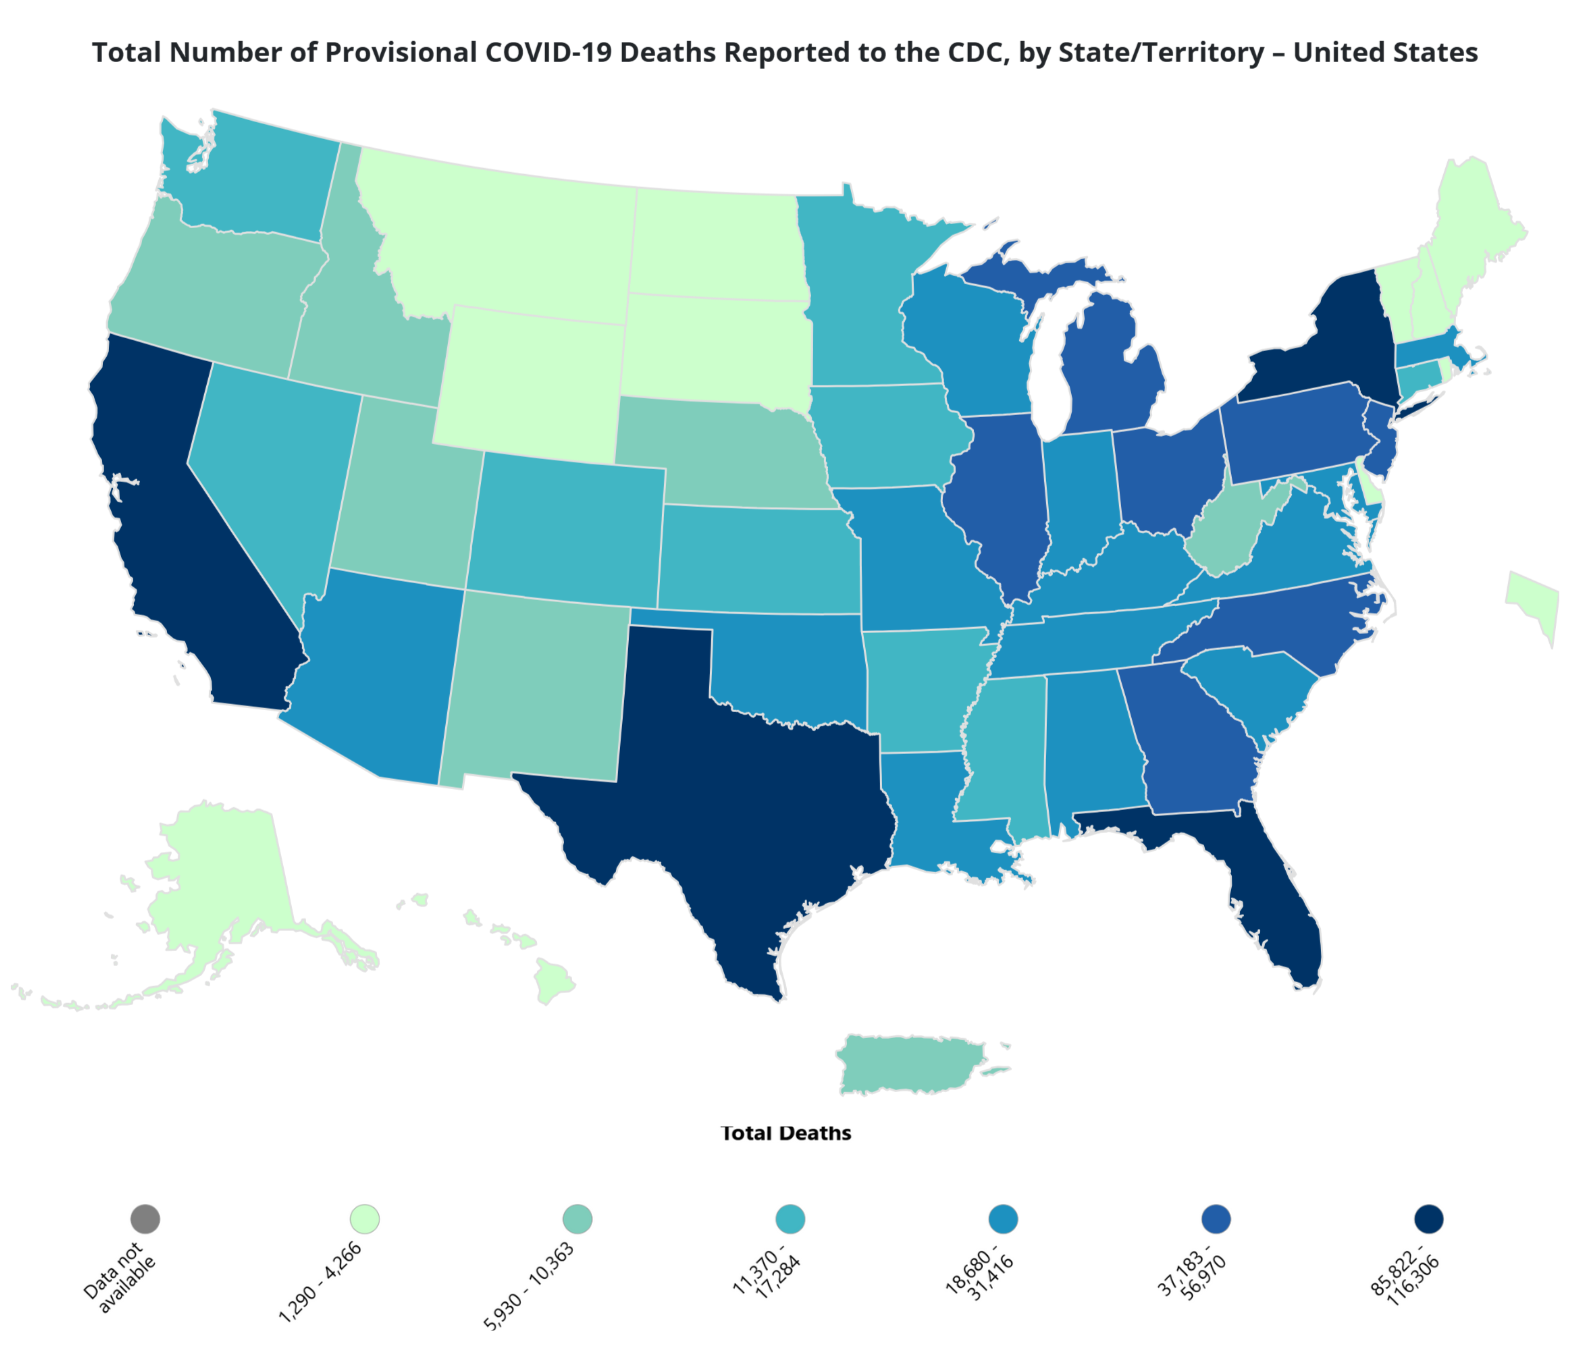
\includegraphics[width=0.95\linewidth]{pics/usCovidDeaths.png}
            \caption{COVID-19 Deaths by Territory per CDC}
        \end{figure}
    \end{minipage}
    \hfill
    \begin{minipage}[t]{0.48\textwidth}
        \begin{block}{Problem Statement}
            \begin{itemize}
                \item Pandemics strain hospital resources, e.g. Florida surpassing 90\% HCF capacity during COVID-19 peaks 
                \item Optimized patient allocation can reduce unmet demand  
                \item Transfers may increase disease spread, but are necessary to alleviate healthcare strain  
                \item Vaccination effects must be implemented
            \end{itemize}           
        \end{block}
    \end{minipage}
    \footnote{\cite{lauer2020incubation} \cite{FloridaHospitalAssociation2021} \cite{CDCCOVIDDataTracker2025}}
\end{frame}

\begin{frame}{Literature Review Map}
    \centering
    \tikzset{
      litbox/.style={
        draw=BraceColor,
        fill=BraceColor!60,
        text=BubbleText,
        rounded corners,
        align=center,
        font=\scriptsize,
        text width=3cm,
        minimum height=1.2cm
      },
      arrow/.style={
        ->, line width=1pt, BraceColor!80,
        shorten >=1pt, shorten <=1pt
      }
    }
    \begin{tikzpicture}[node distance=0.5cm and 1.5cm]
      % Root
      \node[litbox] (root)
        {\textbf{Pandemic Allocation \& Modeling}\\
         Integrates hospital-resource decisions with epidemic dynamics};
  
      % Tier 1: Allocation Optimization
      \node[litbox, below left=of root] (opt)
        {\textbf{Allocation Optimization}\\
         Multi-objective LP balancing ICU/non-ICU and dynamic bed forecasts};
  
      % Tier 1: Epidemiological Modeling
      \node[litbox, below right=of root] (epi)
        {\textbf{Epidemiological Modeling}\\
         Compartmental frameworks capturing immunity, quarantine, and spatial risk};
  
      % Tier 2: Operational Transfer Strategies
      \node[litbox, below=1.5cm of root] (op)
        {\textbf{Operational Transfer Strategies}\\
         Network and queuing models for patient rerouting and surge balancing};
  
      % Tier 3: Mobility Risk Assessment
      \node[litbox, below=of op] (mob)
        {\textbf{Mobility Risk Assessment}\\
         Metapopulation analyses of transfer-induced transmission risk};
  
      % Arrows
      \draw[arrow] (root.south west) -- (opt.north east);
      \draw[arrow] (root.south east) -- (epi.north west);
      \draw[arrow, shorten >=2pt, shorten <=2pt] (root.south)      -- (op.north);
      \draw[arrow] (op.south)        -- (mob.north);
    \end{tikzpicture}

    %\vfill
    \begin{flushleft}
        \tiny
        \cite{aydin2022analyses,dijkstra2023dynamic}\quad
        \cite{li2020modeling,crokidakis2020modeling}\quad
        \cite{della2020network,parker2020optimal}\quad
        \cite{calvetti2021modeling,badr2020association}
    \end{flushleft}
\end{frame}  
    

\section{Case Study: Florida}
\begin{frame}{Study Area \& Data}
    \begin{columns}[c]  % the [c] makes all columns’ contents vertically centered
      \column{0.48\textwidth}
        \centering
        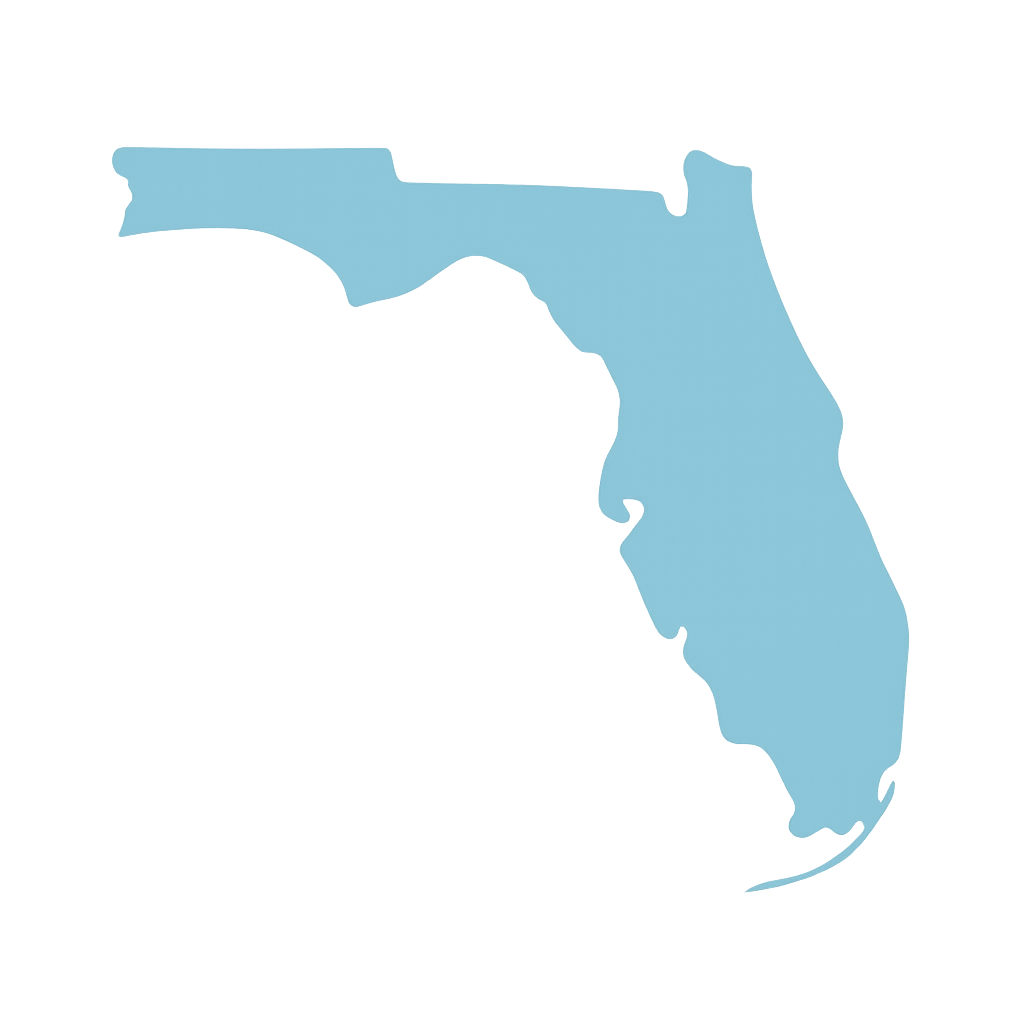
\includegraphics[width=0.85\linewidth]{pics/florida.png}
  
      \column{0.48\textwidth}
        \begin{itemize} 
          \item \textbf{Study Period}: 155 day time horizon
          \item \textbf{Healthcare Facility Data}: \cite{covid19pvi2023}
          \item \textbf{Epidemiological Data}: \cite{abazari2024allocation, florida_covid19_hub2023, zheng2022real}
        \end{itemize}
    \end{columns}
  \end{frame}
  

\section{Model Formulation}

\begin{frame}{Model Component Notation}
    \small
    \begin{minipage}[t]{0.48\textwidth}
        % --- Sets Table ---
        \textbf{Sets} \vspace{1mm}

        \renewcommand{\arraystretch}{1.1}
        \begin{tabular}{|p{0.25\textwidth}|p{0.55\textwidth}|}
            \hline
            $i$ & Regions (counties) \\
            $j$ & Regions (counties) \\
            $t$ & Time periods \\
            $t'$ & Decision periods \\
            \hline
        \end{tabular}
        
        \vspace{5mm}

        % --- Decision Variables Table ---
        \textbf{Decision Variables} \vspace{1mm}

        %\renewcommand{\arraystretch}{1.1}
        \begin{tabular}{|p{0.25\textwidth}|p{0.55\textwidth}|}
            \hline
            $S_i^t, I_i^t, R_i^t, V_i^t$ & SIRV population at time $t$ \\
            $u_i^{t'}$ & Unmet demand \\
            $Z_{ij}^{t'}$ & Transfers $i \to j$ \\
            $\phi_i^{t'}$ & Met demand \\
            $A_{ij}^{t'}$ & Transfer indicator \\
            \hline
        \end{tabular}
    \end{minipage}
    \hfill
    \begin{minipage}[t]{0.48\textwidth}
        % --- Parameters Table ---
        \textbf{Parameters} \vspace{1mm}

        %\renewcommand{\arraystretch}{1.1}
        \begin{tabular}{|p{0.27\textwidth}|p{0.65\textwidth}|}
            \hline
            $S_i^0, I_i^0, R_i^0, V_i^0$ & Initial SIRV populations \\
            $N_i$ & County population \\
            $\beta_i$ & Infection rate \\
            $\gamma_i$ & Recovery rate \\
            $\lambda_i$ & Vaccination rate \\
            $q_i$ & Natural immunity loss rate \\
            $\omega_i$ & Vaccinated immunity loss rate \\
            $\ell_i$ & Leaky vaccine rate \\
            $\alpha_i^{t'}$ & Beds per infection \\
            $d_{ij}$ & Distance between region $i \to j$ \\
            $C_i$ & Healthcare capacity \\
            $n$ & Number of counties \\
            $D$ & Max travel distance \\
            $M$ & A large number \\
            \hline
        \end{tabular}
    \end{minipage}
\end{frame}

%-------------------------------------------------
\begin{frame}{Mathematical Model}
    \footnotesize
    \begin{tikzpicture}[remember picture]
        % ---------- objective + SIRV -------------------------
        \node (sirv) [inner sep=0pt] {
          \begin{minipage}{0.70\textwidth}
          \begin{align*}
              &\min \frac{1}{n}\sum_{i,t'} u_i^{t'} \\[-2pt]
              \text{subject to} \\
              &S_i^{t+1}=S_i^t-\frac{\beta_iS_i^tI_i^t}{N_i}-\lambda_iS_i^t
                         +\omega_iV_i^t+q_iR_i^t &&\forall i,t\\[2pt]
              &I_i^{t+1}=I_i^t+\frac{\beta_iS_i^tI_i^t}{N_i}
                        +\frac{\beta_i\ell_iV_i^{t}I_i^t}{N_i}
                        -\gamma_iI_i^t &&\forall i,t\\[2pt]
              &I_i^{t'+1}=I_i^{t'}+\frac{\beta_iS_i^{t'}I_i^{t'}}{N_i}
                         +\frac{\beta_i\ell_iV_i^{t'}I_i^{t'}}{N_i}
                         -\gamma_iI_i^{t'}+\sum_{j}(Z_{j,i}^{t'}-Z_{i,j}^{t'})
                         &&\forall i,t'\\[2pt]
              &V_i^{t+1}=V_i^t+\lambda_iS_i^{t}-\omega_iV_i^t
                        -\frac{\beta_i\ell_iV_i^tI_i^t}{N_i} &&\forall i,t\\[2pt]
              &R_i^{t+1}=R_i^t+\gamma_iI_i^t-q_iR_i^t &&\forall i,t
          \end{align*}
          \end{minipage}
        };
    
        % ----- tiny brace for the single objective line -----------
        \draw[decorate,decoration={brace,amplitude=6pt},
              draw=BraceColor,very thick]
              ($(sirv.north east)+(1cm,-0.2cm)$) -- ($(sirv.north east)+(1cm,-1.2cm)$)
              node[midway,xshift=1.6cm,
                   fill=BubbleBG,text=BubbleText,
                   rounded corners,inner sep=3pt]
              {\small Objective};
    
        % ----- brace for the 5‑line SIRV dynamics -----------------
        \draw[decorate,decoration={brace,amplitude=6pt},
              draw=BraceColor,very thick]
              ($(sirv.north east)+(1cm,-1.8cm)$) -- ($(sirv.south east)+(1cm,0)$)
              node[midway,xshift=2.0cm,
                   fill=BubbleBG,text=BubbleText,
                   rounded corners,inner sep=3pt]
              {\small SIRV dynamics};
    \end{tikzpicture}
    \end{frame}

\begin{frame}{Mathematical Model (cont.)}
    \footnotesize
    \begin{tikzpicture}[remember picture]
        % --------------- constraints ----------------------------
        \node (cons) [inner sep=0pt] {
          \begin{minipage}{0.70\textwidth}
            \begin{align*}
                &u_i^{t'}=\!\!\!\sum_{t=t'-\psi+1}^{t'}\!\!\alpha_i^{t}I_i^{t}
                            +\!\!\sum_{i\neq j}(Z_{j,i}^{t'}-Z_{i,j}^{t'})
                            -\phi_i^{t'} &&\forall i,t' \\[2pt]
                &\phi_i^{t'}\le\gamma_iC_i &&\forall i,t' \\[6pt]
                %
                &Z_{i,j}^{t'}\le M \cdot A_{i,j}^{t'} &&\forall i,j,t' \\[2pt]
                &Z_{i,j}^{t'}\ge A_{i,j}^{t'} &&\forall i,j,t' \\[6pt]
                &A_{i,j}^{t'} \cdot d_{ij}\le D &&\forall i,j,t' \\[6pt]
                %
                &S_i^t,I_i^t,R_i^t,V_i^t\ge0 &&\forall i,t \\[2pt]
                &u_i^{t'},\phi_i^{t'}\ge0 &&\forall i,t' \\[2pt]
                &Z_{i,j}^{t'}\ge0 &&\forall i,j,t'
            \end{align*}
          \end{minipage}
        };
    
        % ---------- Demand (2 lines) -----------------------------
        \draw[decorate,decoration={brace,amplitude=6pt},
              draw=BraceColor,very thick]
              ($(cons.north east)+(0,-0.5cm)$) -- ($(cons.north east)+(0,-2.1cm)$)
              node[midway,xshift=1.9cm,
                   fill=BubbleBG,text=BubbleText,
                   rounded corners,inner sep=3pt,align=center]
              {\small Unmet \&\\ satisfied demand};
    
        % ---------- Travel (3 lines) -----------------------------
        \draw[decorate,decoration={brace,amplitude=6pt},
              draw=BraceColor,very thick]
              ($(cons.north east)+(0,-2.5cm)$) -- ($(cons.north east)+(0,-4.3cm)$)
              node[midway,xshift=1.9cm,
                   fill=BubbleBG,text=BubbleText,
                   rounded corners,inner sep=3pt,align=center]
              {\small Travel\\ constraints};
    
        % ---------- Non‑negativity (3 lines) ---------------------
        \draw[decorate,decoration={brace,amplitude=6pt},
              draw=BraceColor,very thick]
              ($(cons.north east)+(0,-4.7cm)$) -- ($(cons.south east)+(0,0)$)
              node[midway,xshift=1.9cm,
                   fill=BubbleBG,text=BubbleText,
                   rounded corners,inner sep=3pt,align=center]
              {\small Non-\\negativity};
    \end{tikzpicture}
\end{frame}
    

\begin{frame}{Linearization via McCormick Envelopes}
    \begin{minipage}[t]{0.48\textwidth}
        \begin{itemize}
            \item Nonlinearity arises from $S_i^t I_i^t$ and $V_i^t I_i^t$
            \item We use McCormick envelopes for linearization
            \item Enables more efficient optimization
        \end{itemize}

        % in your beamer frame:
        \centering
        \begin{tikzpicture}[scale=3,>=stealth,font=\scriptsize]
            %--- Theme colors ---
            \definecolor{BGCanvas}{HTML}{36454f}      % slide background (not drawn)
            \definecolor{RegionFill}{HTML}{708090}    % fill color
            \definecolor{Line1}{HTML}{F2F3F4}         % white‑ish (x1+x2=1)
            \definecolor{Line2}{HTML}{97B8C2}         % second constraint (2x1+x2=1)
            \definecolor{Line3}{HTML}{7A9CA7}         % third constraint (x1+2x2=1)
            \definecolor{TextSoft}{HTML}{F2F3F4}      % off‑white text
          
            %--- Feasible region: intersection of x1+x2<=1, 2x1+x2<=1, x1+2x2<=1, x>=0,y>=0 ---
            \fill[RegionFill,opacity=0.6]
              (0,0) --  % origin
              (0,0.5) --               % from x1+2x2=1 at x1=0
              (1/3,1/3) --             % intersection of 2x1+x2=1 & x1+2x2=1
              (0.5,0) --               % from 2x1+x2=1 at x2=0
              cycle;
          
            %--- Constraint lines ---
            %\draw[very thick,Line1] (0,1)   -- (1,0);   % x1 + x2 = 1
            \draw[thick,    Line2] (0,1)   -- (0.5,0); % 2x1 + x2 = 1
            \draw[thick,    Line3] (0,0.5) -- (1,0);   % x1 + 2x2 = 1
            \draw[thick,    Line3] (0,0.75) -- (0.75,0);

            %--- Axes on top ---
            \draw[->, very thick, TextSoft] (0,0) -- (1.2,0) node[anchor=west] {$x_2$};
            \draw[->, very thick, TextSoft] (0,0) -- (0,1.2) node[anchor=south] {$x_1$};
          
            %--- Label inside region ---
            \node[TextSoft,align=center] at (0.19,0.15) {\shortstack{feasible \\region}};
          \end{tikzpicture}
    \end{minipage}
    \hfill
    \begin{minipage}[t]{0.48\textwidth}
        \begin{block}{McCormick Envelopes}
            Let $\min z = xy$, where $x$ and $y$ have bounds $x_l, x_u$ and $y_l, y_u$. Then:
            \begin{align*}
                \min \quad & z \\
                \text{s.t.} \quad
                & z \geq x_l y + x y_l - x_l y_l \\
                & z \geq x_u y + x y_u - x_u y_u \\
                & z \leq x_u y + x y_l - x_u y_l \\
                & z \leq x y_u + x_l y - x_l y_u
            \end{align*}
        \end{block}
    \end{minipage}
    \footnote{\cite{mccormick1976computability}}
\end{frame}
    
    
\section{Results}
\begin{frame}{SIRV vs SIR Dynamics}
    \begin{figure}
        \centering
        \begin{subfigure}{0.43\linewidth}
            \centering
            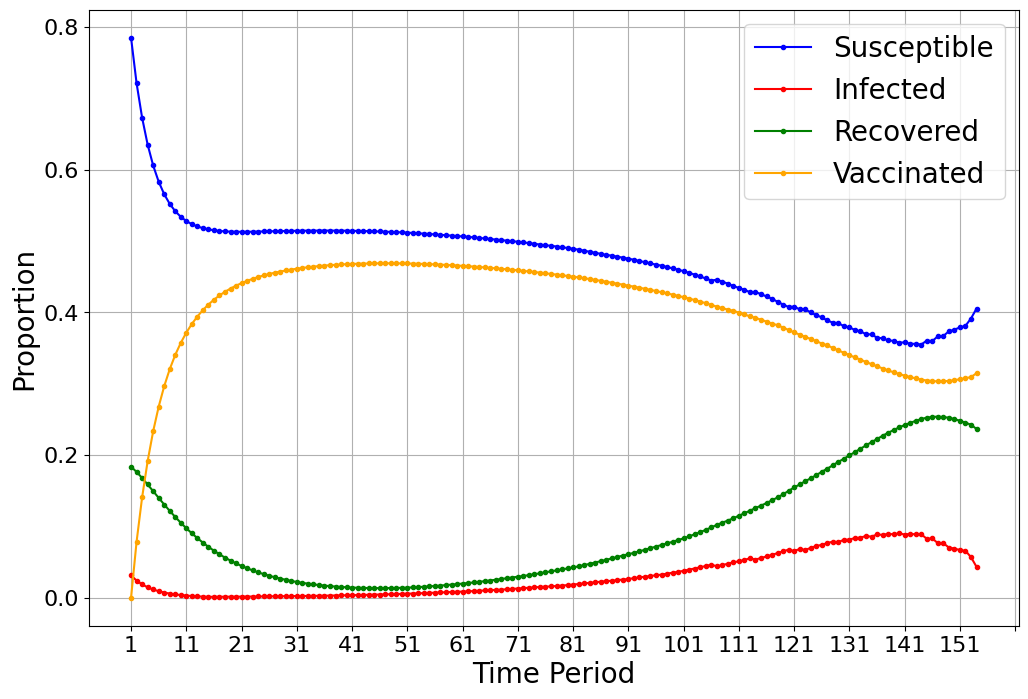
\includegraphics[width=\linewidth]{pics/cumulSIRVDynamicsVax0.1.png}
            \caption{Cumulative SIRV Dynamics}\label{fig:sirvDynamicsVax}
        \end{subfigure}
        \hspace{2em}
        \begin{subfigure}{0.43\linewidth}
            \centering
            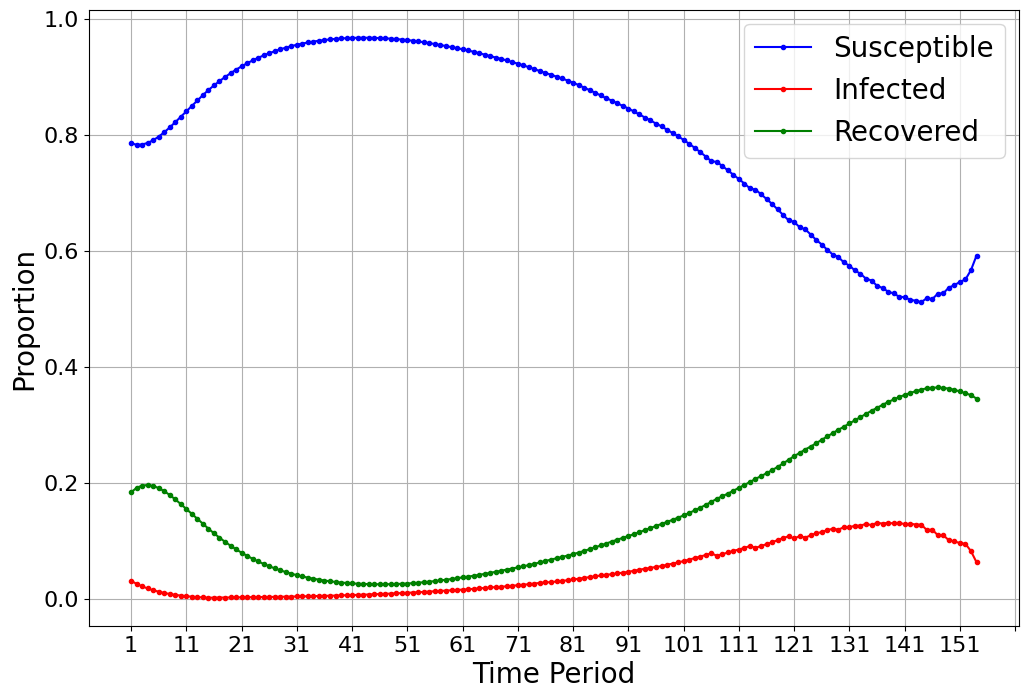
\includegraphics[width=\linewidth]{pics/cumulSIRVDynamicsNoVax.png}
            \caption{Cumulative SIR Dynamics}\label{fig:sirDynamicsNoVax}
        \end{subfigure}
        \caption{Comparison of Cumulative SIRV and SIR Dynamics in Florida}\label{fig:sirvDynamics}
    \end{figure}
\end{frame}

\begin{frame}{Unmet Hospital Demand}
    \begin{figure}
        \centering
        \begin{subfigure}{0.43\linewidth}
            \centering
            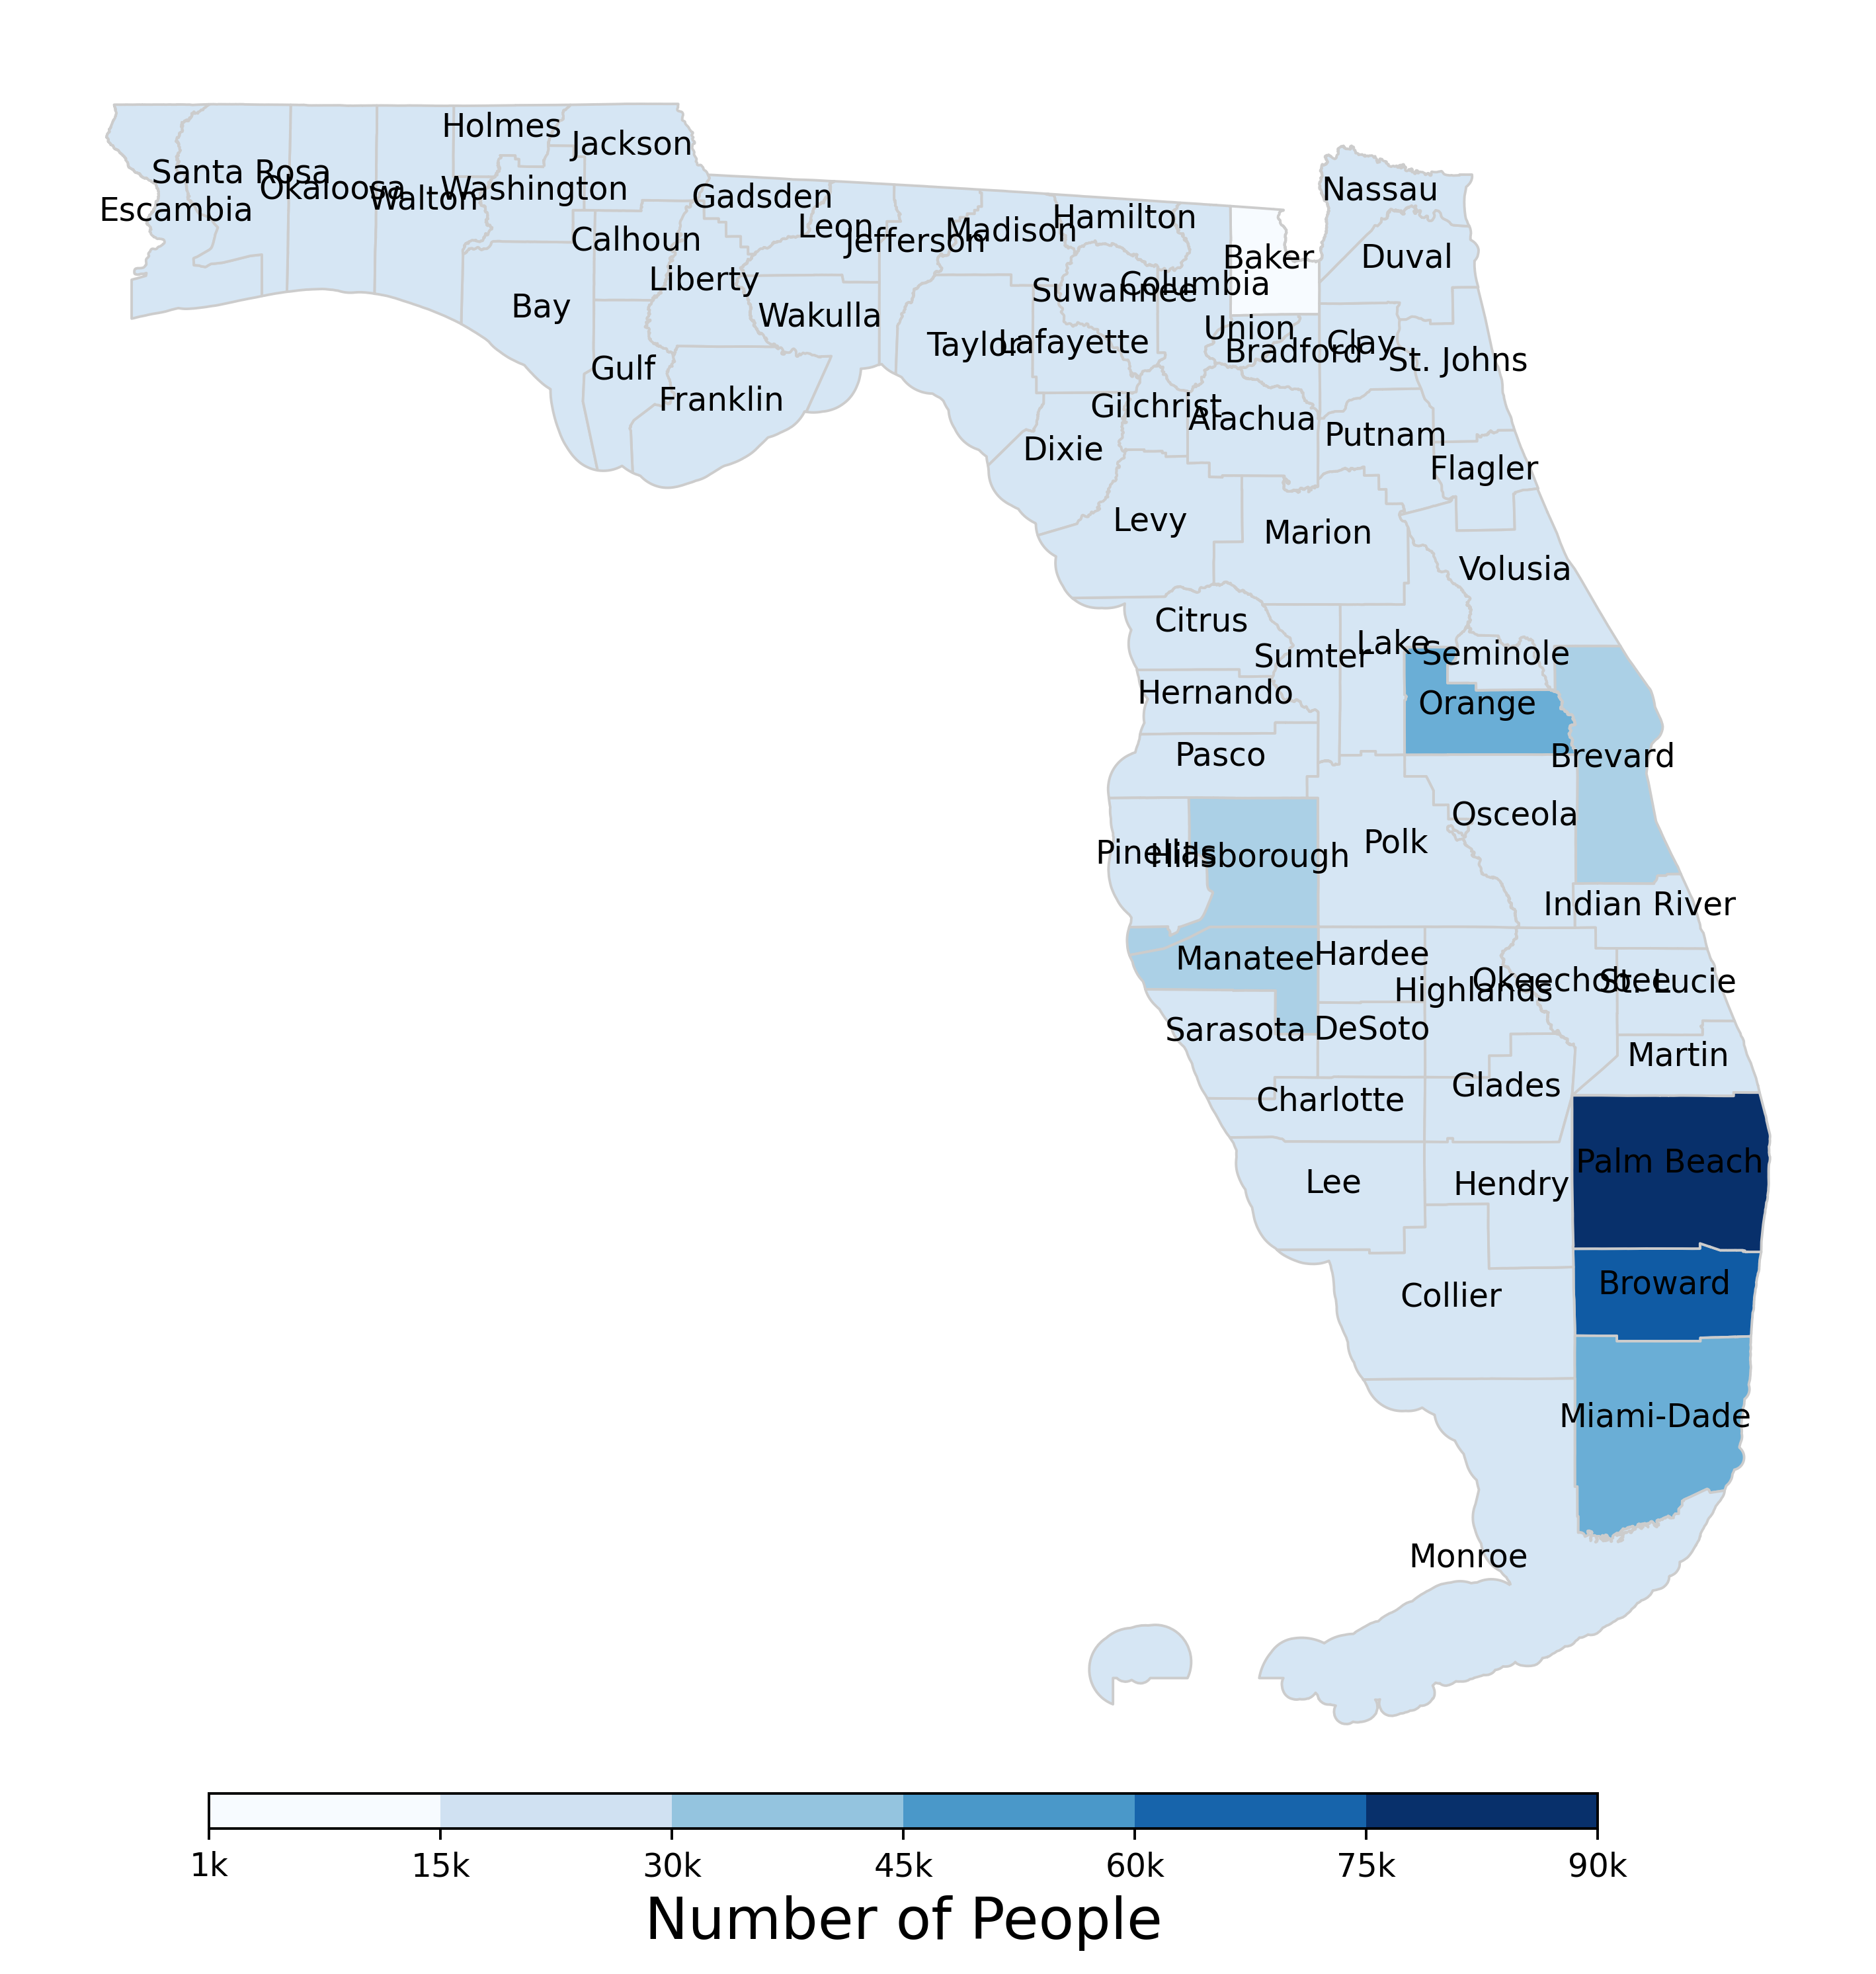
\includegraphics[width=0.85\linewidth]{pics/totalUnmetDemandVax0.1.png}
            \caption{Vaccinated Scenario}\label{fig:udHeatmapVax}
        \end{subfigure}
        \hspace{2em}
        \begin{subfigure}{0.43\linewidth}
            \centering
            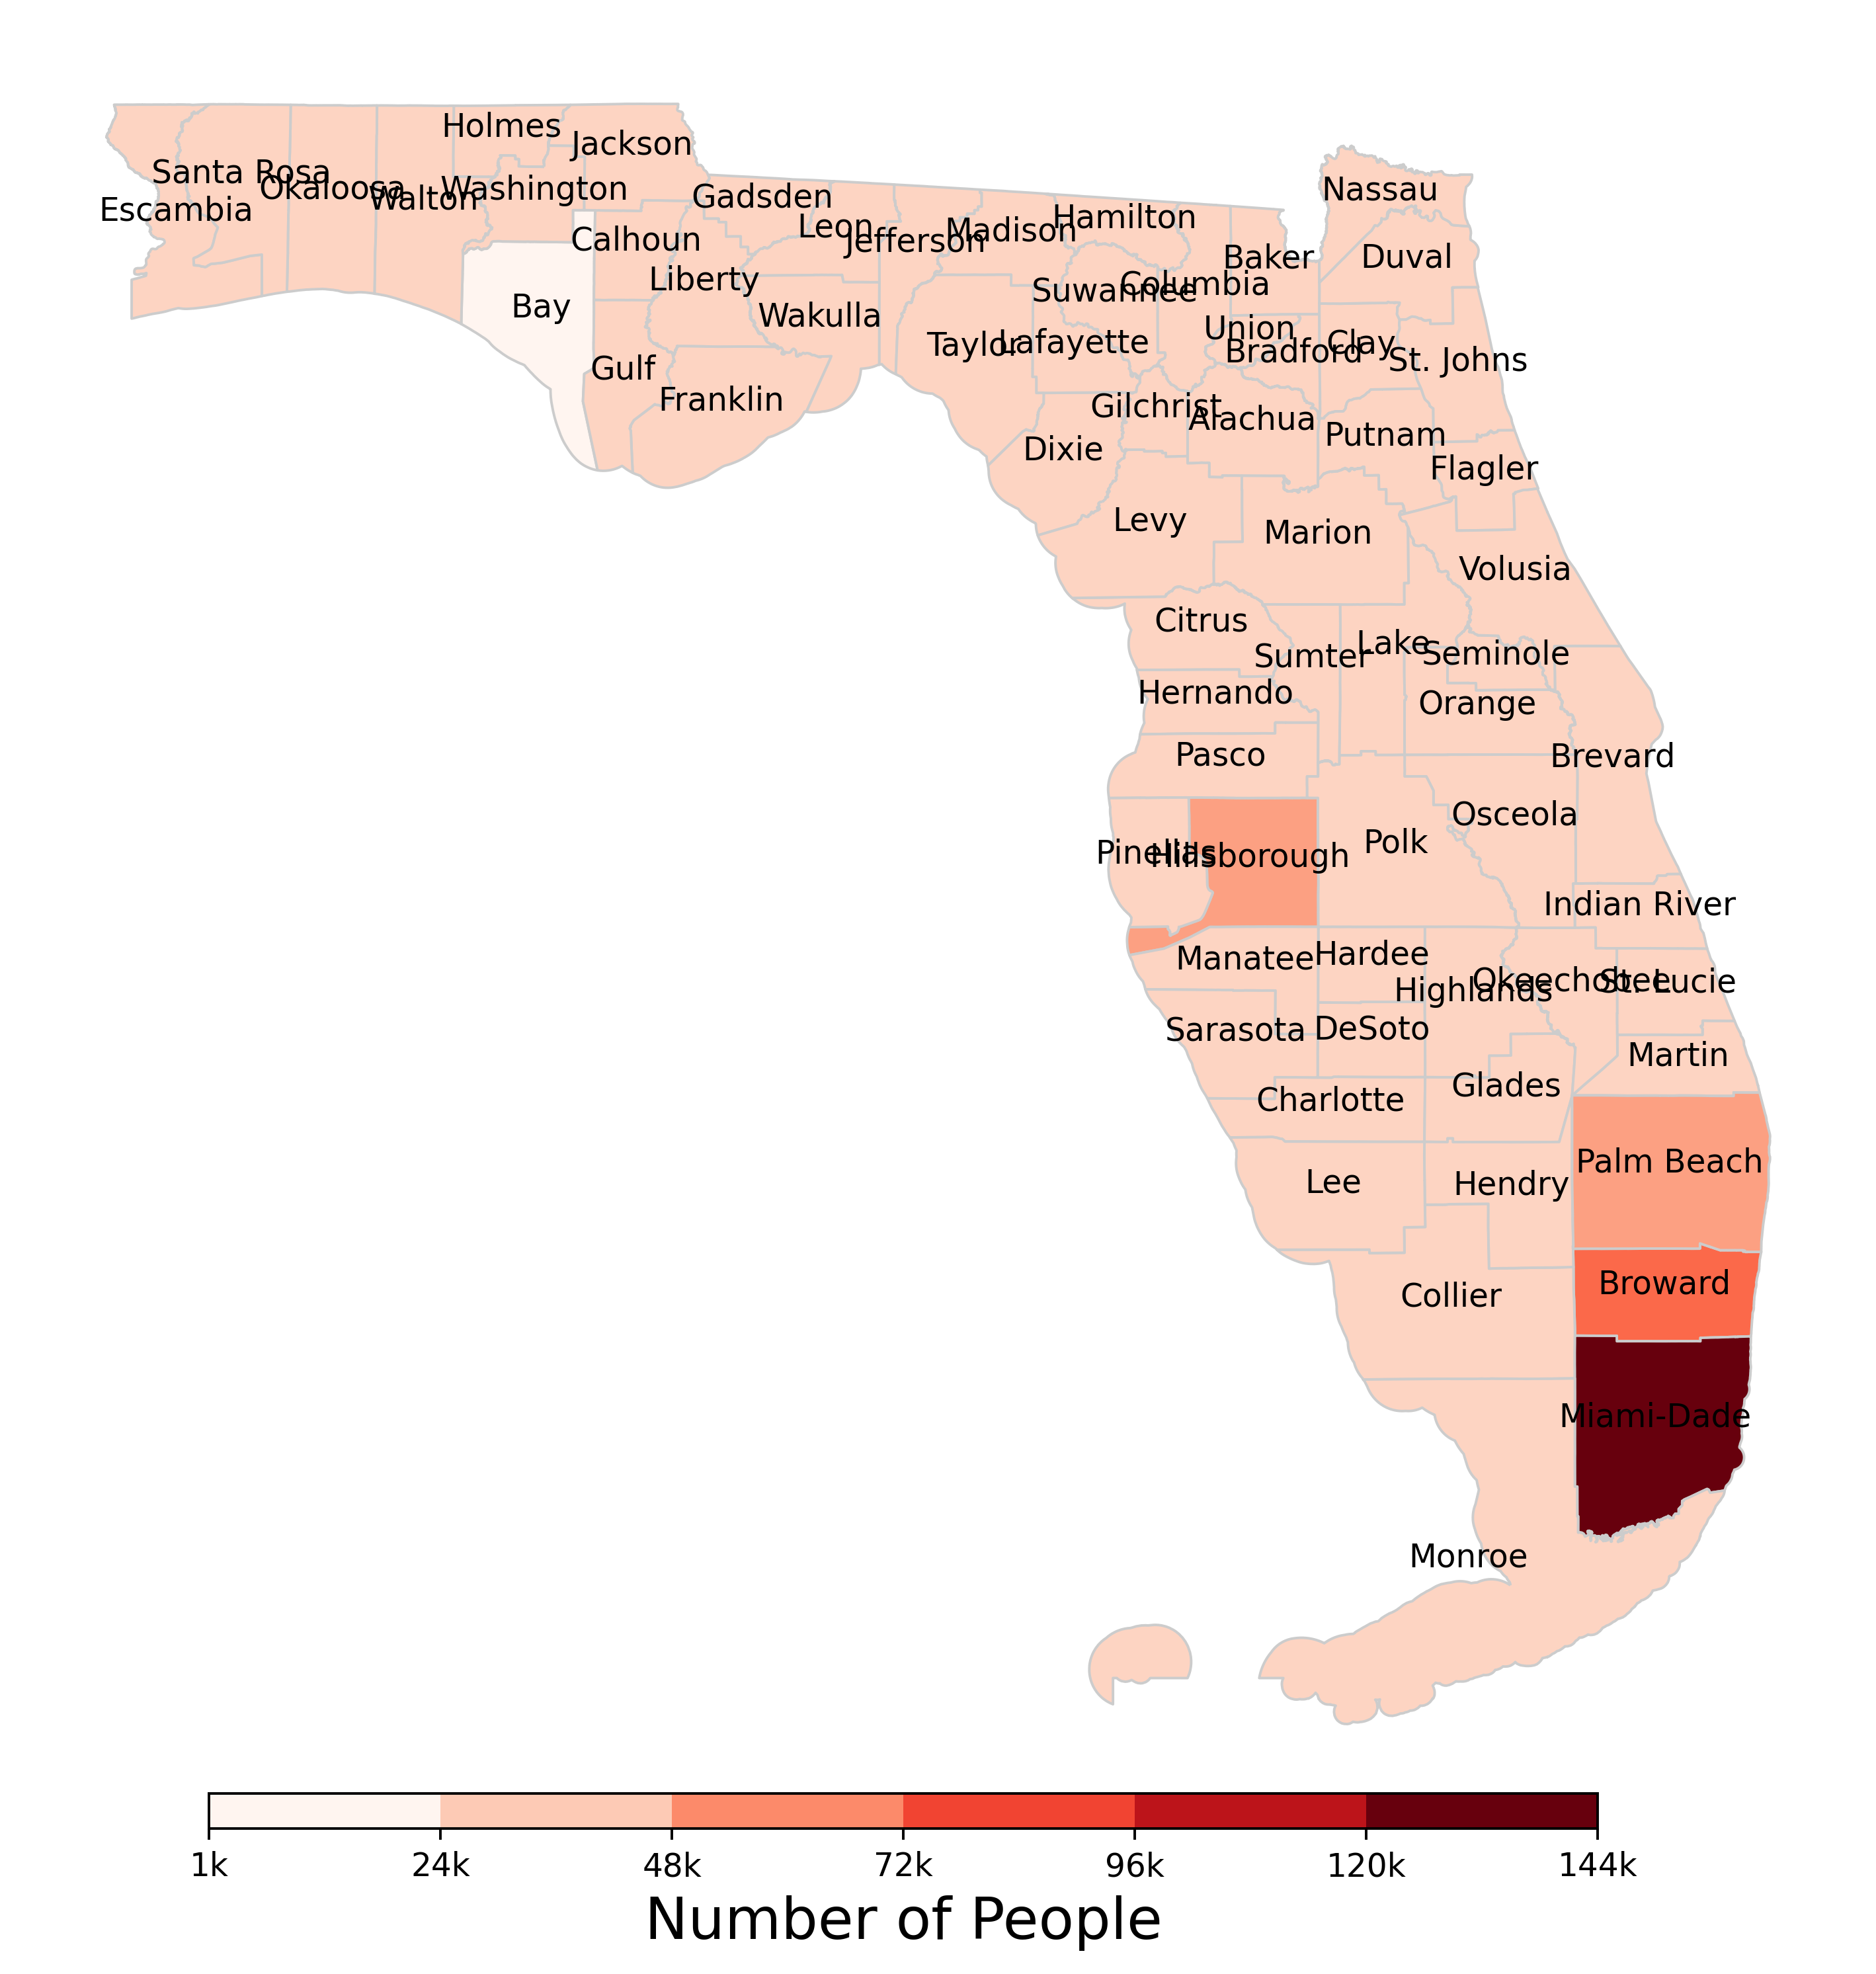
\includegraphics[width=0.85\linewidth]{pics/totalUnmetDemandNoVax.png}
            \caption{Unvaccinated Scenario}\label{fig:udHeatmapNoVax}
        \end{subfigure}
        \caption{Comparison of Aggregate Unmet Demand in Vaccinated vs. Unvaccinated Scenarios}\label{fig:udHeatmap}
    \end{figure}
\end{frame}

\begin{frame}{Patient Transfers}
    \begin{figure}[h]
        \centering
        \begin{subfigure}{0.445\linewidth}
            \centering
            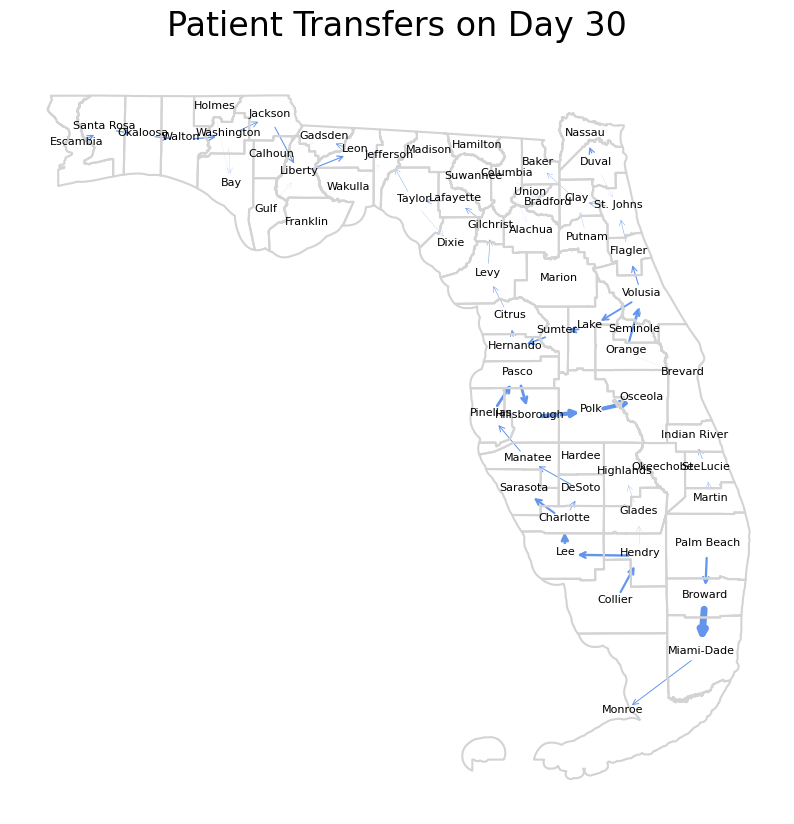
\includegraphics[width=0.85\linewidth]{pics/travel_day_30_Vax0.1.png}
            \caption{Vaccinated Scenario (Day 30)}\label{fig:patientAllocVax}
        \end{subfigure}
        \hspace{2em}
        \begin{subfigure}{0.445\linewidth}
            \centering
            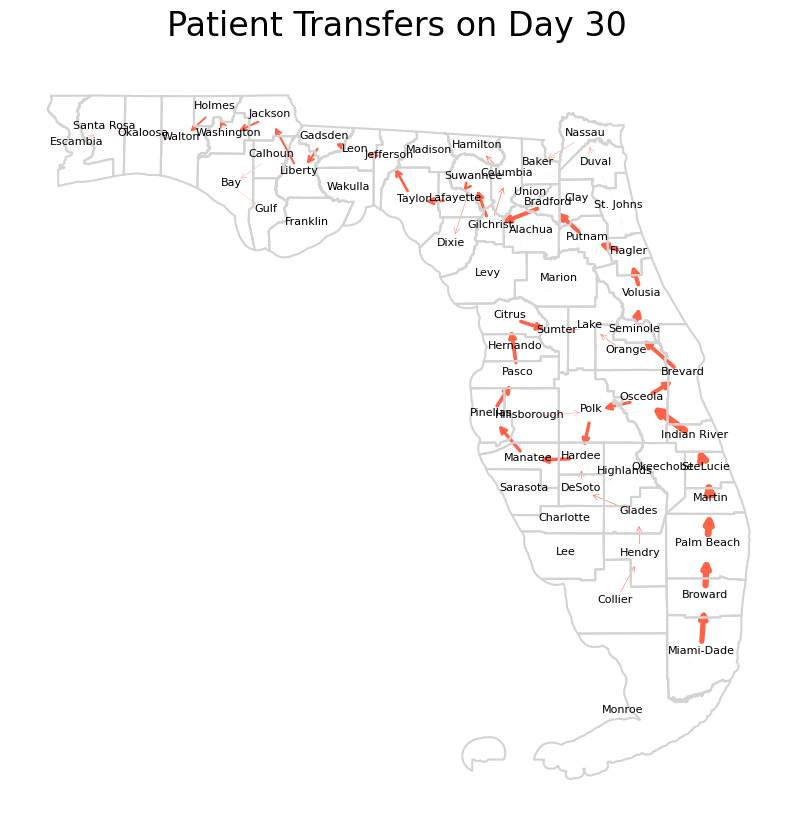
\includegraphics[width=0.85\linewidth]{pics/travel_day_30_NoVax.png}
            \caption{Unvaccinated Scenario (Day 30)}\label{fig:patientAllocNoVax}
        \end{subfigure}
        \caption{Comparison of Patient Allocation in Vaccinated vs. Unvaccinated Scenarios}\label{fig:patientAlloc}
    \end{figure}
\end{frame}

\section{Implications}
\begin{frame}{Policy Recommendations}
    \begin{itemize}
        \item Prioritize vaccine distribution in urban hotspots and adjust strategy as transmission shifts
        \item Use boosters and ongoing monitoring to maintain protection as immunity wanes
        \item Coordinate hospital transfers and strengthen infrastructure in  high-demand areas
    \end{itemize}
    
\end{frame}

\section{Conclusion}
\begin{frame}{Key Conclusions and Future Work}
    \begin{minipage}[t]{0.48\textwidth}
        \begin{block}{Conclusions}
            \begin{itemize}
                \item Coordinated vaccine and patient transfer strategies reduce hospital strain
                \item Urban regions tend to receive transfers; rural areas more often send patients
                \item Vaccination mitigates surges but waning immunity can trigger secondary waves
            \end{itemize}
        \end{block}
    \end{minipage}
    \hfill
    \begin{minipage}[t]{0.48\textwidth}
        \begin{block}{Future Work}
            \begin{itemize}
                \item Incorporate demographics and socioeconomic factors into disease modeling
                \item Explicitly model vaccine supply, logistics, and effects with real data
                \item Refine patient transfer rules to reduce chaining and improve realism
                \item Dyanamic disease parameters
            \end{itemize}
        \end{block}
    \end{minipage}
\end{frame}
    

\begin{frame}[allowframebreaks]{References}
    \tiny
    \bibliography{references.bib}
    \bibliographystyle{apalike}
\end{frame}
 
\begin{frame}
    \Huge{\centerline{\textbf{Questions?}}}
\end{frame}

\end{document}